\chapter{Anexo I: Matriz de Consistencia}


\begin{table}[h!]
	\centering
	\small
	\begin{tabular}{ |m{5cm}|m{5cm}|m{5cm}|  }
		\hline
		\rowcolor{bluejean}
		\Centering \color{white}{PROBLEMAS}& \Centering \color{white}{OBJETIVOS}& \Centering \color{white}{HIPÓTESIS}\\
		\hline
		\rowcolor{turq}
		\Centering Problema General& \Centering Objetivo General & \Centering Hipótesis General \\
		\hline
		{\ProblemaGeneral} & { \ObjetivoGeneral} & {\HipotesisGeneral} \\
		\hline
		\rowcolor{turq}
		\Centering Problemas Específicos& \Centering Objetivos Específicos & \Centering Hipótesis Específicas \\
		\hline
		{\Pbone} & {\Objone} & {\Hone} \\
		\hline
		{\Pbtwo} & {\Objtwo} & {\Htwo} \\
		\hline
		{\Pbthree} & {\Objthree} & {\Hthree} \\
		\hline
		{\Pbfour} & {\Objfour} & {\Hfour} \\
		\hline

	\end{tabular}
	\caption{Matriz de consistencia. Fuente: Elaboración propia}
	\label{1:table}
\end{table}

\begin{table}[htbp]
    \centering
    \begin{tabular}{|p{4.5cm}|p{4.5cm}|p{6cm}| }
        \toprule
        \Centering \textbf{Hipótesis Específica} & \Centering \textbf{Indicadores} & \Centering \textbf{Fórmulas} \\
        \midrule
        {\Hone} & 
        \begin{tabular}[t]{@{}p{4.3cm}@{}}
%            $*$Porcentaje de integración de APIs \\
            $*$Calidad de datos\\
	     $*$Tiempo de respuesta de la API\\
	     $*$Porcentaje de consultas resueltas
        \end{tabular} & 
        \begin{tabular}[t]{@{}p{5.8cm}@{}}
%		$\frac{\text{Número de APIs integradas}}{\text{Total de APIs disponibles}} \times 100$\\\\
            $\frac{\text{\tiny Cantidad de datos precisos y actualizados}}{\text{\tiny Total de datos utilizados}} \times 100$\\\\
            $\frac{\text{Tiempo total de respuesta de la API}}{\text{Número total de consultas}}$\\\\
		$\frac{\text{Consultas resueltas}}{\text{Total de consultas realizadas}} \times 100$
        \end{tabular} \\
        \midrule
         {\Htwo}  & 
        \begin{tabular}[t]{@{}p{4.3cm}@{}}
            $*$Precisión del modelo de lenguaje natural \\
            $*$Eficiencia del chatbot\\\\
		$*$Precisión de Diagnóstico (PD)\\
		$*$Tasa de Error del Sistema (TES)
        \end{tabular} & 
        \begin{tabular}[t]{@{}p{5.8cm}@{}}
            $\frac{\text{Número de respuestas correctas}}{\text{Total de respuestas generadas}} \times 100$\\\\
            $\frac{\text{Número de consultas manejadas}}{\text{Tiempo total de prueba}}$\\\\
            $\frac{\text{\tiny Número de diagósticos correctos}}{\text{\tiny Número Total de diagósticos}} \times {\tiny 100}$\\\\
		$\frac{\text{Número de errores del sistema}}{\text{ Número total de interacciones}} \times 100$
        \end{tabular} \\
        \midrule
        {\Hthree} & 
        \begin{tabular}[t]{@{}p{4.3cm}@{}}
            $*$Exactitud del conjunto de datos de entrenamiento \\\break
%            $*$Tasa de generalización del modelo\\
		$*$Precisión de la validación cruzada\\
		$*$Tasa de Mejoría en Entrenamiento (TME)
        \end{tabular} & 
        \begin{tabular}[t]{@{}p{5.8cm}@{}}
            $\frac{\text{\tiny Número de pares de consulta-respuesta correctos}}{\text{\tiny Total de pares de consulta-respuesta}} \times 100$\\\\\\\break
%            $\frac{\text{\tiny Número de consultas generales respondidas correctamente}}{\text{\tiny Total de consultas generales}} \times {\tiny 100}$\\
            $\frac{\text{\tiny Número de consultas validadas correctamente}}{\text{\tiny Total de consultas validadas}} \times 100$\\\\
		$\frac{\text{\tiny Error inicial - Error final}}{\text{\tiny Error inicial}} \times 100$
        \end{tabular} \\
        \midrule
        {\Hfour} & 
        \begin{tabular}[t]{@{}p{4.3cm}@{}}
            $*$Reducción en tiempos de espera \\\\
            $*$Aumento en la accesibilidad de servicios médicos\\
	     $*$Cobertura de Usuarios en Áreas Rurales (CUAR)\\\\
	     $*$Satisfacción del usuario
        \end{tabular} & 
        \begin{tabular}[t]{@{}p{5.8cm}@{}}
		\tiny Antes= Tiempo promedio de espera antes del chatbot \break
		\tiny Despues= Tiempo promedio de espera después del chatbot\\
            $\frac{\text{\tiny Antes} - \text{\tiny Despues}}{\text{\tiny Antes}} \times 100$ \\\\
		$\frac{\text{\tiny Número de consultas médicas atendidas por el chatbot}}{\text{\tiny Total de consultas médicas realizadas}} \times 100$\\\\\\
	      $\frac{\text{\tiny Número de usuarios en áreas rurales}}{\text{\tiny Número total de usuarios}} \times 100$\\\\\\
		$\frac{\text{Número de usuarios satisfechos}}{\text{Total de usuarios encuestados}} \times 100$
        \end{tabular} \\
        \bottomrule
    \end{tabular}
 \caption{Tabla de Hipótesis Específicas, Indicadores y Fórmulas}
    \label{tab:hipotesis}
\end{table}
\vspace{-5mm}

\chapter{Anexo II: Arbol del Problema}
%\section{Conclusiones}

\begin{figure}[H]
	\begin{center}
		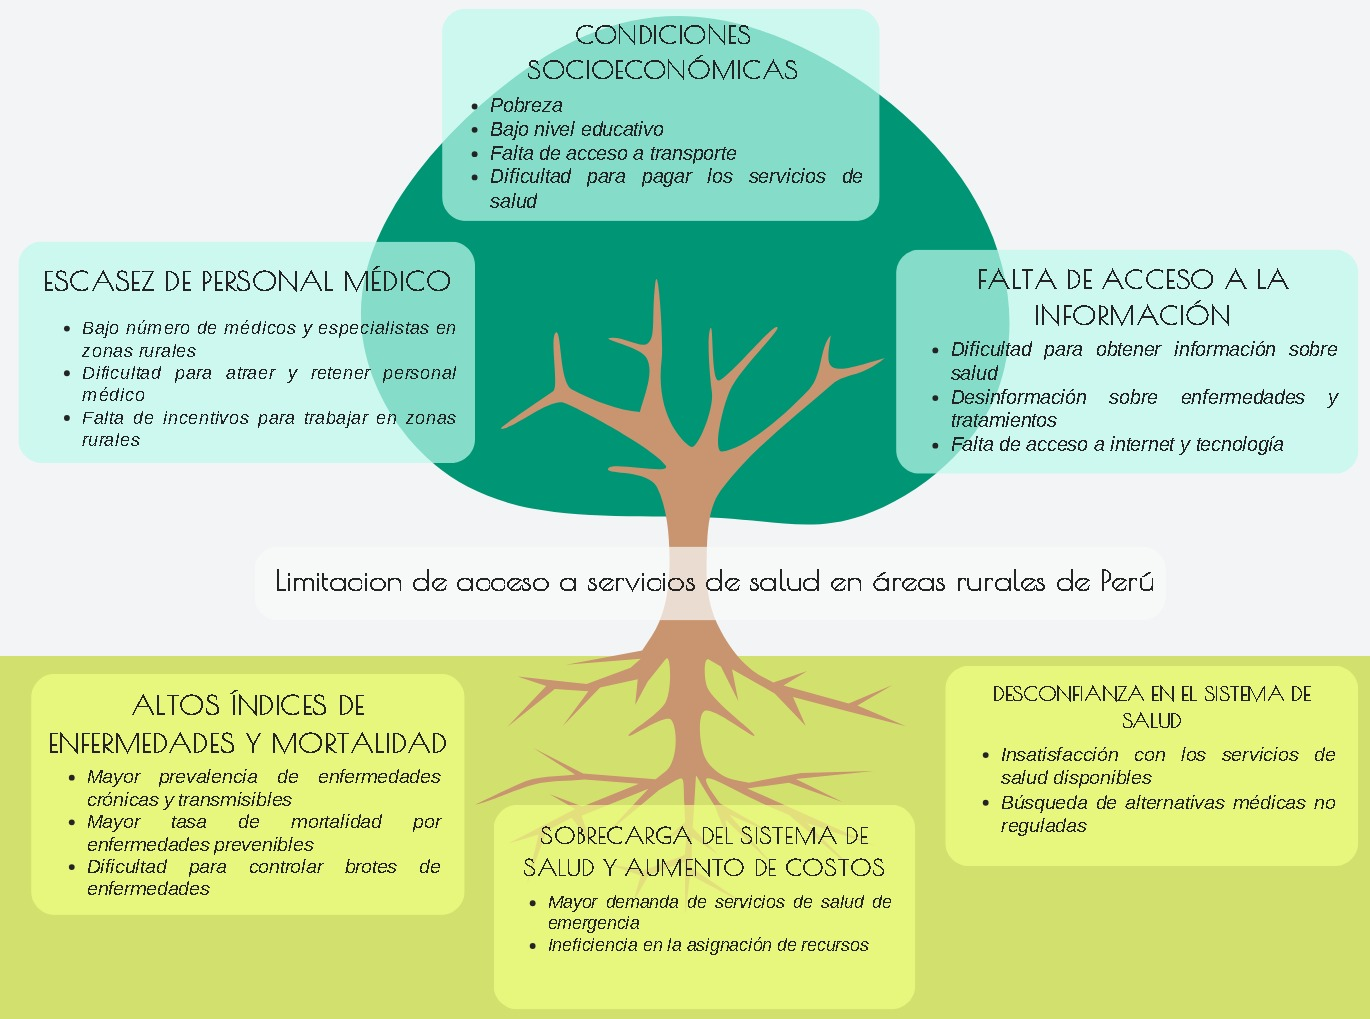
\includegraphics[width=0.8\textwidth]{images_repo/Arbol del problema.jpeg}
		\caption{Árbol del problema. Fuente: Elaboración propia}
		\label{1:fig}
	\end{center}
\end{figure}
\vspace{-120mm}
\chapter{Anexo IV: Resumen de Papers investigados}
%\section{Conclusiones}
\vspace{-5mm}


\begin{table}[H]
	\newcommand{\multirot}[1]{\multirow{2}{*}[-8ex]{\rotcell{\rlap{#1}}}}
	%\scriptsize
	\footnotesize
	\centering
	\begin{tabular}{|m{0.5cm}|m{0.3cm}|m{4cm}|m{2cm}|m{0.6cm}|m{1.7cm}|m{3cm}|} 
		\hline
		\rowcolor[rgb]{0,0.251,0.502} \multicolumn{1}{|c|}{\textcolor{white}{Tipo}} & \multicolumn{1}{c|}{\textcolor{white}{N°}} & \multicolumn{1}{c|}{\textcolor{white}{Título}}                                                                             & \multicolumn{1}{c|}{\textcolor{white}{Autor}}        & \multicolumn{1}{c|}{\textcolor{white}{Año}} & \multicolumn{1}{c|}{\textcolor{white}{País}} & \multicolumn{1}{c|}{\textcolor{white}{Fuente}}                                                        \\ 
		\hline
		\multirot{Problema}                                        & 1                                             & \citetitle{HealthChatBots-2022}                                                                     & \citeauthor{HealthChatBots-2022}           &\citeyear{HealthChatBots-2022}                                         
		& Ver el pais despues                              
		&    \citeurl{HealthChatBots-2022}                                                                           \\ 
		\cline{2-7}
		& 2               
		& \citetitle{peftmedaware_2023}                                              
		& \citeauthor{peftmedaware_2023}                    
		& \citeyear{peftmedaware_2023}                                       
		& Ver el pais despues                                  
		& \citeurl{peftmedaware_2023}\\ 
		\hline
		\multirow{3}{*}[-10ex]{\rotcell{\rlap{Propuesta}}}
		& 3                    
		& \citetitle{Medbot-2020}                                                   
		& \citeauthor{Medbot-2020}                    
		& \citeyear{Medbot-2020}                                       
		& Ver el pais                                   
		& \citeurl{Medbot-2020}\\  
		\cline{2-7}
		& 4                                            
		& \citetitle{IntelligentChatbot_2020}                               
		& \citeauthor{IntelligentChatbot_2020}                    
		& \citeyear{IntelligentChatbot_2020}                                       
		& Ver el                                  
		&\citeurl{IntelligentChatbot_2020}\\
		\cline{2-7}
		& 5                                             &\citetitle{HHHAnOnlineMedical}                                                   
		&\citeauthor{HHHAnOnlineMedical}                    
		&\citeyear{HHHAnOnlineMedical}                                       
		& Ver                                
		&\citeurl{HHHAnOnlineMedical}\\
		
		\hline
		\multirow{4}{*}[-20ex]{\rotcell{\rlap{Técnica}}}                                          & 6                                          
		& \citetitle{HealFavor}                                              
		& \citeauthor{HealFavor}                    
		& \citeyear{HealFavor}                                   
		&  despues                                  
		& \citeurl{HealFavor}   \\ 
		\cline{2-7}
		& 7                                             & \citetitle{chatdoctor}                                              
		& \citeauthor{chatdoctor}                    
		& \citeyear{chatdoctor}                                   
		& Ver el pais despues                                  
		& \citeurl{chatdoctor}   \\ 
		\hline
	\end{tabular}
	\caption{Cuadro Resumen de Papers investigados. Fuente: Elaboración propia}
\label{A:table}
\end{table}

\begin{longtable}{|m{0.5cm}|m{0.3cm}|m{4cm}|m{2cm}|m{0.6cm}|m{1.7cm}|m{3cm}|}
	\hline
	\rowcolor[rgb]{0,0.251,0.502} \multicolumn{1}{|c|}{\textcolor{white}{Tipo}} & \multicolumn{1}{c|}{\textcolor{white}{N°}} & \multicolumn{1}{c|}{\textcolor{white}{Título}} & \multicolumn{1}{c|}{\textcolor{white}{Autor}} & \multicolumn{1}{c|}{\textcolor{white}{Año}} & \multicolumn{1}{c|}{\textcolor{white}{País}} & \multicolumn{1}{c|}{\textcolor{white}{Fuente}} \\
	\hline
	\endfirsthead
	
	\hline
	\rowcolor[rgb]{0,0.251,0.502} \multicolumn{1}{|c|}{\textcolor{white}{Tipo}} & \multicolumn{1}{c|}{\textcolor{white}{N°}} & \multicolumn{1}{c|}{\textcolor{white}{Título}} & \multicolumn{1}{c|}{\textcolor{white}{Autor}} & \multicolumn{1}{c|}{\textcolor{white}{Año}} & \multicolumn{1}{c|}{\textcolor{white}{País}} & \multicolumn{1}{c|}{\textcolor{white}{Fuente}} \\
	\hline
	\endhead
	
	\hline \multicolumn{7}{r}{{Continúa en la siguiente página}} \\
	\endfoot
	
	\hline
	\endlastfoot
	
	\multirow{4}{*}[-2.5ex]{\rotcell{Técnica}}
	& 8 & \citetitle{AutoResponse-2022} & \citeauthor{AutoResponse-2022} & \citeyear{AutoResponse-2022} & Ver el pais después & \citeurl{AutoResponse-2022}  \\
	\cline{2-7}
	& 9 & \citetitle{ApproachtoMedical} & \citeauthor{ApproachtoMedical} & \citeyear{ApproachtoMedical} & Ver el pais después & \citeurl{ApproachtoMedical} \\
	\cline{2-7}
	& 10 & \citetitle{MedicalChatBot} & \citeauthor{MedicalChatBot} & \citeyear{MedicalChatBot} & Ver el pais después & \citeurl{MedicalChatBot} \\
	\hline
\end{longtable}



